% Options for packages loaded elsewhere
% Options for packages loaded elsewhere
\PassOptionsToPackage{unicode}{hyperref}
\PassOptionsToPackage{hyphens}{url}
%
\documentclass[
  english,
  russian,
  12pt,
  a4paper,
  DIV=11,
  numbers=noendperiod]{scrreprt}
\usepackage{xcolor}
\usepackage{amsmath,amssymb}
\setcounter{secnumdepth}{5}
\usepackage{iftex}
\ifPDFTeX
  \usepackage[T1]{fontenc}
  \usepackage[utf8]{inputenc}
  \usepackage{textcomp} % provide euro and other symbols
\else % if luatex or xetex
  \usepackage{unicode-math} % this also loads fontspec
  \defaultfontfeatures{Scale=MatchLowercase}
  \defaultfontfeatures[\rmfamily]{Ligatures=TeX,Scale=1}
\fi
\usepackage{lmodern}
\ifPDFTeX\else
  % xetex/luatex font selection
\fi
% Use upquote if available, for straight quotes in verbatim environments
\IfFileExists{upquote.sty}{\usepackage{upquote}}{}
\IfFileExists{microtype.sty}{% use microtype if available
  \usepackage[]{microtype}
  \UseMicrotypeSet[protrusion]{basicmath} % disable protrusion for tt fonts
}{}
\usepackage{setspace}
% Make \paragraph and \subparagraph free-standing
\makeatletter
\ifx\paragraph\undefined\else
  \let\oldparagraph\paragraph
  \renewcommand{\paragraph}{
    \@ifstar
      \xxxParagraphStar
      \xxxParagraphNoStar
  }
  \newcommand{\xxxParagraphStar}[1]{\oldparagraph*{#1}\mbox{}}
  \newcommand{\xxxParagraphNoStar}[1]{\oldparagraph{#1}\mbox{}}
\fi
\ifx\subparagraph\undefined\else
  \let\oldsubparagraph\subparagraph
  \renewcommand{\subparagraph}{
    \@ifstar
      \xxxSubParagraphStar
      \xxxSubParagraphNoStar
  }
  \newcommand{\xxxSubParagraphStar}[1]{\oldsubparagraph*{#1}\mbox{}}
  \newcommand{\xxxSubParagraphNoStar}[1]{\oldsubparagraph{#1}\mbox{}}
\fi
\makeatother


\usepackage{longtable,booktabs,array}
\usepackage{calc} % for calculating minipage widths
% Correct order of tables after \paragraph or \subparagraph
\usepackage{etoolbox}
\makeatletter
\patchcmd\longtable{\par}{\if@noskipsec\mbox{}\fi\par}{}{}
\makeatother
% Allow footnotes in longtable head/foot
\IfFileExists{footnotehyper.sty}{\usepackage{footnotehyper}}{\usepackage{footnote}}
\makesavenoteenv{longtable}
\usepackage{graphicx}
\makeatletter
\newsavebox\pandoc@box
\newcommand*\pandocbounded[1]{% scales image to fit in text height/width
  \sbox\pandoc@box{#1}%
  \Gscale@div\@tempa{\textheight}{\dimexpr\ht\pandoc@box+\dp\pandoc@box\relax}%
  \Gscale@div\@tempb{\linewidth}{\wd\pandoc@box}%
  \ifdim\@tempb\p@<\@tempa\p@\let\@tempa\@tempb\fi% select the smaller of both
  \ifdim\@tempa\p@<\p@\scalebox{\@tempa}{\usebox\pandoc@box}%
  \else\usebox{\pandoc@box}%
  \fi%
}
% Set default figure placement to htbp
\def\fps@figure{htbp}
\makeatother



\ifLuaTeX
\usepackage[bidi=basic,provide=*]{babel}
\else
\usepackage[bidi=default,provide=*]{babel}
\fi
% get rid of language-specific shorthands (see #6817):
\let\LanguageShortHands\languageshorthands
\def\languageshorthands#1{}


\setlength{\emergencystretch}{3em} % prevent overfull lines

\providecommand{\tightlist}{%
  \setlength{\itemsep}{0pt}\setlength{\parskip}{0pt}}



 
\usepackage[style=gost-numeric,backend=biber,langhook=extras,autolang=other*]{biblatex}
\addbibresource{bib/cite.bib}

\usepackage[]{csquotes}

\usepackage{indentfirst}
\usepackage{float}
\floatplacement{figure}{H}
\IfFileExists{plex-otf.sty}{
  %% Full TeXlive
  \usepackage[
    % math,
    RM={Scale=0.94},SS={Scale=0.94},SScon={Scale=0.94},TT={Scale=MatchLowercase,FakeStretch=0.9},
    DefaultFeatures={Ligatures=Common}
  ]{plex-otf}
  % \usepackage[Scale=MatchUppercase]{juliamono}
}{
  %% TinyTeX
  \usepackage{libertine}
}
\KOMAoption{captions}{tableheading}
\makeatletter
\@ifpackageloaded{caption}{}{\usepackage{caption}}
\AtBeginDocument{%
\ifdefined\contentsname
  \renewcommand*\contentsname{Содержание}
\else
  \newcommand\contentsname{Содержание}
\fi
\ifdefined\listfigurename
  \renewcommand*\listfigurename{Список иллюстраций}
\else
  \newcommand\listfigurename{Список иллюстраций}
\fi
\ifdefined\listtablename
  \renewcommand*\listtablename{Список таблиц}
\else
  \newcommand\listtablename{Список таблиц}
\fi
\ifdefined\figurename
  \renewcommand*\figurename{Рисунок}
\else
  \newcommand\figurename{Рисунок}
\fi
\ifdefined\tablename
  \renewcommand*\tablename{Таблица}
\else
  \newcommand\tablename{Таблица}
\fi
}
\@ifpackageloaded{float}{}{\usepackage{float}}
\floatstyle{ruled}
\@ifundefined{c@chapter}{\newfloat{codelisting}{h}{lop}}{\newfloat{codelisting}{h}{lop}[chapter]}
\floatname{codelisting}{Список}
\newcommand*\listoflistings{\listof{codelisting}{Листинги}}
\makeatother
\makeatletter
\makeatother
\makeatletter
\@ifpackageloaded{caption}{}{\usepackage{caption}}
\@ifpackageloaded{subcaption}{}{\usepackage{subcaption}}
\makeatother
\usepackage{bookmark}
\IfFileExists{xurl.sty}{\usepackage{xurl}}{} % add URL line breaks if available
\urlstyle{same}
\hypersetup{
  pdftitle={Прохождение внешнего курса. Этап 3},
  pdfauthor={Мещерякова София Андреевна},
  pdflang={ru-RU},
  hidelinks,
  pdfcreator={LaTeX via pandoc}}


\title{Прохождение внешнего курса. Этап 3}
\usepackage{etoolbox}
\makeatletter
\providecommand{\subtitle}[1]{% add subtitle to \maketitle
  \apptocmd{\@title}{\par {\large #1 \par}}{}{}
}
\makeatother
\subtitle{Продвинутые темы}
\author{Мещерякова София Андреевна}
\date{}
\begin{document}
\maketitle

\renewcommand*\contentsname{Содержание}
{
\setcounter{tocdepth}{1}
\tableofcontents
}
\listoffigures
\listoftables

\setstretch{1.5}
\chapter{Цель
работы}\label{ux446ux435ux43bux44c-ux440ux430ux431ux43eux442ux44b}

Выполнить третий этап курса \enquote{Введение в Linux}. Освоить
продвинуты темы для работы в ОС Linux.

\chapter{Выполнение
заданий}\label{ux432ux44bux43fux43eux43bux43dux435ux43dux438ux435-ux437ux430ux434ux430ux43dux438ux439}

\section{Текстовый редактор
vim}\label{ux442ux435ux43aux441ux442ux43eux432ux44bux439-ux440ux435ux434ux430ux43aux442ux43eux440-vim}

Чтобы выйти без сохранения, нужно перейти в режим команд строки (:),
ввести q (quit) и нажать Enter (рис.~\ref{fig-001}).

\begin{figure}

\centering{


\includegraphics[width=0.7\linewidth,height=\textheight,keepaspectratio]{image3/1.png}

}

\caption{\label{fig-001}}

\end{figure}%

word --- это последовательность букв, цифр и знаков подчеркивания (\_)
ИЛИ последовательность других символов (знаков препинания). WORD --- это
любая последовательность символов, разделенная исключительно пробелами
или символами табуляции/конца строки.(рис.~\ref{fig-002}).

\begin{figure}

\centering{


\includegraphics[width=0.7\linewidth,height=\textheight,keepaspectratio]{image3/2.png}

}

\caption{\label{fig-002}}

\end{figure}%

Исходная строка: one two three four five Цель: three four four four five
(курсор изначально на первой букве o).

\begin{itemize}
\item
  xxxxxxxxwywPpxxxxxxxx: удаляет 8 символов поочередно (one two ).
  Строка становится three four five, курсор на t.w: перемещает курсор на
  four.yw: копирует (yank) слово four с пробелом.P: вставляет
  скопированное перед four (получается four four).p: вставляет еще раз
  после (получается four four four).
\item
  d2wwywPpd2w: удаляет два слова (one и two ). Строка: three four
  five.w: прыгает на слово four.yw: копирует four .P и p: вставляют его
  до и после текущего слова, доводя количество four до трёх.
\item
  d2wwifour four d2w: удаляет one two . Строка: three four five.w:
  перемещает курсор на слово four.ifour four : переходит в режим вставки
  перед словом и дописывает нехватающие four four
\item
  d2w\(bifour four <Esc>d2w: удаляет one two . Строка: three four five.\):
  прыгает в самый конец строки (на слово five).b: возвращается назад на
  одно слово (на four).ifour four : вставляет текст перед ним.
\item
  ddithree four four four five dd: полностью удаляет всю текущую
  строку.ithree four four four five : переходит в режим вставки в пустую
  строку и просто пишет требуемый текст целиком с нуля.
  (рис.~\ref{fig-003}).
\end{itemize}

\begin{figure}

\centering{


\includegraphics[width=0.7\linewidth,height=\textheight,keepaspectratio]{image3/3.png}

}

\caption{\label{fig-003}}

\end{figure}%

:\%s --- замена во всех строках, шаблон Windows, замена Linux. Без флага
g заменяется только первое вхождение в строке. Enter не входит в команду
(рис.~\ref{fig-004}).

\begin{figure}

\centering{


\includegraphics[width=0.7\linewidth,height=\textheight,keepaspectratio]{image3/4.png}

}

\caption{\label{fig-004}}

\end{figure}%

\begin{itemize}
\tightlist
\item
  Выйти из режима выделения можно, нажав клавишу Esc два раза (Иногда
  достаточно и одного нажатия, но двойной Esc гарантированно возвращает
  в нормальный режим из любого состояния).
\item
  В режиме выделения можно использовать команды перемещения (например,
  W, e, \$, и др.) (При перемещении курсора выделенная область будет
  автоматически расширяться или сужаться).
\item
  В режиме выделения можно использовать команды d (удалить) и y
  (скопировать) (Они применятся ко всему тексту, который попал в область
  выделения).
\item
  Режим выделения открывается из нормального режима по нажатию
  \enquote{v} (Маленькая v включает посимвольный визуальный режим, V ---
  построчный, а Ctrl+V --- блочный).
\item
  Когда вы находитесь в режиме выделения, внизу редактора горит надпись
  -- VISUAL -- (или -- ВИЗУАЛЬНЫЙ РЕЖИМ --)
\end{itemize}

Почему не подходит оставшийся вариант:

\begin{itemize}
\tightlist
\item
  Чтобы выйти из режима выделения, нужно ввести :q --- Это неверно.
  Команда :q используется в командном режиме для выхода из самого
  редактора Vim, а не для смены режимов (рис.~\ref{fig-005}).
\end{itemize}

\begin{figure}

\centering{


\includegraphics[width=0.7\linewidth,height=\textheight,keepaspectratio]{image3/5.png}

}

\caption{\label{fig-005}}

\end{figure}%

\section{Скрипты на bash:
основы}\label{ux441ux43aux440ux438ux43fux442ux44b-ux43dux430-bash-ux43eux441ux43dux43eux432ux44b}

История команд привязана к текущей оболочке. Запуск новой оболочки (sh,
затем bash) даёт новую историю (рис.~\ref{fig-006}).

\begin{figure}

\centering{


\includegraphics[width=0.7\linewidth,height=\textheight,keepaspectratio]{image3/6.png}

}

\caption{\label{fig-006}}

\end{figure}%

Команда cd меняет директорию только внутри скрипта, но файл создаётся в
/home/bi/ (рис.~\ref{fig-007}).

\begin{figure}

\centering{


\includegraphics[width=0.7\linewidth,height=\textheight,keepaspectratio]{image3/7.png}

}

\caption{\label{fig-007}}

\end{figure}%

Правила именования переменных в bash (рис.~\ref{fig-008}):

\begin{enumerate}
\def\labelenumi{\arabic{enumi}.}
\tightlist
\item
  Имя должно состоять только из букв (a-z, A-Z), цифр (0-9) и знаков
  подчеркивания (\_).
\item
  Имя может начинаться только с буквы или со знака подчеркивания. Цифра
  на первом месте недопустима.
\item
  Символы пробела, точек, знаков доллара или коммерческого «at» (@) в
  именах переменных запрещены.
\end{enumerate}

не подходят варианты:

\begin{itemize}
\tightlist
\item
  var i able --- содержит пробелы.
\item
  var.i.able --- содержит точки.
\item
  variab\$\$le --- содержит знаки \$.
\item
  var@iable --- содержит символ @.
\end{itemize}

\begin{figure}

\centering{


\includegraphics[width=0.7\linewidth,height=\textheight,keepaspectratio]{image3/8.png}

}

\caption{\label{fig-008}}

\end{figure}%

\$1 и \$2 --- аргументы скрипта. Чтобы вывести символ \$ как текст, его
нужно экранировать \$. Первый вариант (\$1=\$1) выведет \$1=значение
(рис.~\ref{fig-009}).

\begin{figure}

\centering{


\includegraphics[width=0.7\linewidth,height=\textheight,keepaspectratio]{image3/9.png}

}

\caption{\label{fig-009}}

\end{figure}%

\section{Скрипты на bash: ветвления и
циклы}\label{ux441ux43aux440ux438ux43fux442ux44b-ux43dux430-bash-ux432ux435ux442ux432ux43bux435ux43dux438ux44f-ux438-ux446ux438ux43aux43bux44b}

Верные:

\begin{itemize}
\tightlist
\item
  5 -ge 5
\item
  -s \$0
\item
  \$\# -ge 0
\item
  -e \$0
\item
  ! (4 -le 3)
\end{itemize}

Неверно: * \$\# -gt 0 --- Условие истинно только тогда, когда количество
аргументов строго больше нуля (-gt, greater than). Если запустить скрипт
вообще без параметров, это условие вернет ложь (рис.~\ref{fig-010}).

\begin{figure}

\centering{


\includegraphics[width=0.7\linewidth,height=\textheight,keepaspectratio]{image3/10.png}

}

\caption{\label{fig-010}}

\end{figure}%

Правильным вариантом ответа является:

\begin{itemize}
\tightlist
\item
  Сначала four, потом four (рис.~\ref{fig-011}).
\end{itemize}

В скрипте используются следующие числовые операторы сравнения:

\begin{itemize}
\tightlist
\item
  -gt (greater than) --- строго больше.
\item
  -lt (less than) --- строго меньше.
\item
  -eq (equal) --- равно.
\end{itemize}

\begin{enumerate}
\def\labelenumi{\arabic{enumi}.}
\tightlist
\item
  Первый запуск при var = 3:
\end{enumerate}

\begin{itemize}
\tightlist
\item
  if {[}{[} 3 -gt 5 {]}{]} ➔ Ложь (3 не больше 5).
\item
  elif {[}{[} 3 -lt 3 {]}{]} ➔ Ложь (3 не меньше 3, они равны).
\item
  elif {[}{[} 3 -eq 4 {]}{]} ➔ Ложь (3 не равно 4).
\item
  Выполняется ветка else ➔ выводится four.
\end{itemize}

\begin{enumerate}
\def\labelenumi{\arabic{enumi}.}
\setcounter{enumi}{1}
\tightlist
\item
  Второй запуск при var = 5:
\end{enumerate}

\begin{itemize}
\tightlist
\item
  if {[}{[} 5 -gt 5 {]}{]} ➔ Ложь (5 не больше 5, они равны).
\item
  elif {[}{[} 5 -lt 3 {]}{]} ➔ Ложь (5 не меньше 3).
\item
  elif {[}{[} 5 -eq 4 {]}{]} ➔ Ложь (5 не равно 4).
\item
  Снова выполняется ветка else ➔ выводится four.
\end{itemize}

\begin{figure}

\centering{


\includegraphics[width=0.7\linewidth,height=\textheight,keepaspectratio]{image3/11.png}

}

\caption{\label{fig-011}}

\end{figure}%

Конструкция проверяет число студентов и выводит нужное сообщение. Для
2--4 выводится число с \enquote{students}. Для 0 особая строка. Для 5 и
больше --- \enquote{A lot of students} (рис.~\ref{fig-012}).

\begin{verbatim}
if [[ $1 -eq 1 ]]; then
    echo "$1 student"
elif [[ $1 -gt 1 && $1 -le 4 ]]; then
    echo "$1 students"
elif [[ $1 -ge 5 ]]; then
    echo "A lot of students"
else
    echo "No students"
fi
\end{verbatim}

\begin{figure}

\centering{


\includegraphics[width=0.7\linewidth,height=\textheight,keepaspectratio]{image3/12.png}

}

\caption{\label{fig-012}}

\end{figure}%

Цикл for перебирает три строки: \enquote{a,}, \enquote{b,} и
\enquote{c\_d}. continue пропускает вывод \enquote{finish} для строк,
которые лексикографически больше \enquote{c}. \enquote{c\_d}
\textgreater{} \enquote{c}, поэтому для неё \enquote{finish} не
выводится. Остальные строки выводят и \enquote{start}, и
\enquote{finish}. Итог: \enquote{start} --- 5 раз, \enquote{finish} ---
4 раза (рис.~\ref{fig-013}).

\begin{figure}

\centering{


\includegraphics[width=0.7\linewidth,height=\textheight,keepaspectratio]{image3/13.png}

}

\caption{\label{fig-013}}

\end{figure}%

Бесконечный цикл while true. При пустом имени или возрасте 0 --- выход с
bye. Иначе определение группы (рис.~\ref{fig-014}).

\begin{verbatim}
# put your shell (bash) code here
child=16
adult=25
s=0

while [[ $s != 1 ]]
    do
        echo "enter your name: "
        read name
    if [[ -z $name ]]; then
        echo "bye"
        s=1
    elif [[ -n $name ]]; then
        echo "enter your age: "
        read age
        if [[ $age -eq 0 ]]; then
            echo "bye"
            s=1
        elif [[ $age -le $child ]]; then
            echo "$name, your group is child"
        elif [[ $age -gt $adult ]]; then
             echo "$name, your group is adult"
        else 
            echo "$name, your group is youth"
        fi
    fi
done
\end{verbatim}

\begin{figure}

\centering{


\includegraphics[width=0.7\linewidth,height=\textheight,keepaspectratio]{image3/14.png}

}

\caption{\label{fig-014}}

\end{figure}%

\section{Скрипты на bash:
разное}\label{ux441ux43aux440ux438ux43fux442ux44b-ux43dux430-bash-ux440ux430ux437ux43dux43eux435}

Команда let в bash создана специально для вычисления арифметических
выражений. Она автоматически интерпретирует текст как математическую
операцию и позволяет опускать знак доллара \$ перед именами переменных:

\begin{enumerate}
\def\labelenumi{\arabic{enumi}.}
\tightlist
\item
  let a=a+b и let a=\(a+\)b --- классический синтаксис без пробелов.
\item
  let \enquote{a+=b} и let \enquote{a=\(a+\)b} --- использование двойных
  кавычек позволяет безопасно экранировать специальные символы (включая
  пробелы, если бы они там были), при этом bash успешно раскрывает
  значения переменных внутри кавычек.
\end{enumerate}

\begin{itemize}
\tightlist
\item
  a=\(a+\)b --- без встроенной математической команды (вроде let или
  конструкции \$((\ldots))) bash воспринимает это выражение как обычное
  сложение строк. Вместо числа 15 в переменную a запишется строка 10+5
  (рис.~\ref{fig-015}).
\end{itemize}

\begin{figure}

\centering{


\includegraphics[width=0.7\linewidth,height=\textheight,keepaspectratio]{image3/15.png}

}

\caption{\label{fig-015}}

\end{figure}%

Команда echo \enquote{\enquote*{pwd}} выводит текущую директорию,
результат выполнения pwd (рис.~\ref{fig-016}).

\begin{figure}

\centering{


\includegraphics[width=0.7\linewidth,height=\textheight,keepaspectratio]{image3/16.png}

}

\caption{\label{fig-016}}

\end{figure}%

Правильными утверждениями и конструкциями в bash являются следующие
варианты:

\begin{itemize}
\item
  if \program\texttt{\textgreater{}\ some\_file.txt}
\item
  Сначала запустить program, затем if {[}{[} \$? -eq 0 {]}{]}

  \begin{enumerate}
  \def\labelenumi{\arabic{enumi}.}
  \tightlist
  \item
    **if
    \program\texttt{\textgreater{}\ some\_file.txt**\ Перенаправление\ вывода\ \textgreater{}\ some\_file.txtперехватывает\ весь\ текст,\ который\ программа\ пишет\ вstdout,\ и\ убирает\ его\ с\ экрана,\ сохраняя\ в\ файл.\ При\ этом\ конструкция\ if}
    по-прежнему проверяет именно код возврата самой программы (если он
    равен 0, условие выполнится).
  \item
    Сначала запустить program, затем if {[}{[} \$? -eq 0 {]}{]} Это
    классический и самый надежный способ. Переменная \$? автоматически
    сохраняет код возврата последней выполненной команды. Вы можете
    запустить программу привычным образом, а следующей строкой
    проверить, завершилась ли она успешно (код 0).
  \end{enumerate}
\end{itemize}

остальные варианты:

\begin{itemize}
\tightlist
\item
  **Сначала
  var=\program\texttt{,\ затем\ if\ {[}{[}\ \$var\ -eq\ 0\ {]}{]}**\ —\ Косая\ кавычка\ (backtick)\ сохраняет\ в\ переменную\ var**текстовый\ вывод**\ программы\ (stdout),\ а\ не\ код\ её\ завершения.\ Если\ программа\ выведет\ слово\ "Привет",\ условие{[}{[}\ "Привет"\ -eq\ 0\ {]}{]}}
  вызовет ошибку или отработает некорректно.
\item
  **if {[}{[}
  \program\texttt{-eq\ 0\ {]}{]}**\ —\ По\ той\ же\ причине:\ внутри\ {[}{[}\ ...\ {]}{]}}
  будет сравниваться число 0 и текстовый вывод программы, а не код
  возврата (рис.~\ref{fig-017}).
\end{itemize}

\begin{figure}

\centering{


\includegraphics[width=0.7\linewidth,height=\textheight,keepaspectratio]{image3/17.png}

}

\caption{\label{fig-017}}

\end{figure}%

В функции counter переменная c1 объявлена как local, поэтому её значение
не сохраняется между вызовами --- после десяти вызовов c1 остаётся
пустой. Нелокальная переменная c2 накапливает сумму:
2*(1+2+\ldots+10)=110. Команда echo выводит \enquote{counters are and
110} (между are и and --- два пробела) (рис.~\ref{fig-018}).

\begin{figure}

\centering{


\includegraphics[width=0.7\linewidth,height=\textheight,keepaspectratio]{image3/18.png}

}

\caption{\label{fig-018}}

\end{figure}%

Бесконечный цикл чтения двух чисел. Пустая строка --- выход. Функция gcd
реализует алгоритм Евклида (рис.~\ref{fig-019}).

\begin{verbatim}
# put your shell (bash) code here
while [ true ] 
do
    read n1 n2
if [ -z $n1]; then
    echo "bye"
    break
else 
    gcd () {
    r=1
    if [ $n2 -eq 0 ]
    then
    echo "bye"
    fi
    while [ $r -ne 0 ]
    do
    r=$((n1%n2))
    n1=$n2
    n2=$r
    done
    }
    gcd $1 $2
    echo "GCD is $n1"
fi
done
\end{verbatim}

\begin{figure}

\centering{


\includegraphics[width=0.7\linewidth,height=\textheight,keepaspectratio]{image3/19.png}

}

\caption{\label{fig-019}}

\end{figure}%

\$((exp)) вычисляет арифметическое выражение. Если выражение неверно ---
ошибка и выход. exit --- выход с bye (рис.~\ref{fig-020}).

\begin{verbatim}
# put your shell (bash) code here
while [[ true ]]
do
    read a zn b
    if [[ $a == "exit" ]]
    then 
        echo "bye"
        break
    elif [[ "$a" =~ "^[0-9]+$" &&  "$b" =~ "^[0-9]+$" ]]
    then 
        echo "error"
        break
    else
        case $zn in
        "+") let "res = a + b";;
        "-") let "res = a - b";;
        "*") let "res = a * b";;
        "/") let "res = a / b";;
        "%") let "res = a % b";;
        "**") let "res = a ** b";;
        *) echo "error"; break ;;
        esac
        echo "$res"
    fi
done
\end{verbatim}

\begin{figure}

\centering{


\includegraphics[width=0.7\linewidth,height=\textheight,keepaspectratio]{image3/20.png}

}

\caption{\label{fig-020}}

\end{figure}%

\section{Продвинутый поиск и
редактирование}\label{ux43fux440ux43eux434ux432ux438ux43dux443ux442ux44bux439-ux43fux43eux438ux441ux43a-ux438-ux440ux435ux434ux430ux43aux442ux438ux440ux43eux432ux430ux43dux438ux435}

-iname ищет без учёта регистра, -name --- с учётом (рис.~\ref{fig-021}).

\begin{figure}

\centering{


\includegraphics[width=0.7\linewidth,height=\textheight,keepaspectratio]{image3/21.png}

}

\caption{\label{fig-021}}

\end{figure}%

-path ищет по полному пути, -name только по имени. В некоторых случаях
(файл в текущей директории) результат совпадёт, но не всегда
(рис.~\ref{fig-022}).

\begin{figure}

\centering{


\includegraphics[width=0.7\linewidth,height=\textheight,keepaspectratio]{image3/22.png}

}

\caption{\label{fig-022}}

\end{figure}%

Команда find с параметрами -mindepth 2 -maxdepth 3 ищет файлы на глубине
2 и 3 относительно /home/bi/. file1 находится на глубине 2
(/home/bi/dir1/file1), file2 --- на глубине 3
(/home/bi/dir1/dir2/file2), file3 --- на глубине 4
(/home/bi/dir1/dir2/dir3/file3). Будут найдены file1 и file2 --- все,
кроме file3 (рис.~\ref{fig-023}).

\begin{figure}

\centering{


\includegraphics[width=0.7\linewidth,height=\textheight,keepaspectratio]{image3/23.png}

}

\caption{\label{fig-023}}

\end{figure}%

Во всех вариантах grep выводит одинаковое количество строк, так как
каждая строка файла содержит слово \enquote{word}. Опции -A, -B, -C
добавляют контекст, но поскольку искомая строка есть в каждой строке,
добавленные строки контекста совпадают с уже выводимыми. В итоге все
команды создадут файл results.txt одинакового размера
(рис.~\ref{fig-024}).

\begin{figure}

\centering{


\includegraphics[width=0.7\linewidth,height=\textheight,keepaspectratio]{image3/24.png}

}

\caption{\label{fig-024}}

\end{figure}%

Регулярное выражение ищет строки, которые оканчиваются на buntu. Перед
buntu может быть буква u или цифра 0, а перед ними --- необязательный
символ из указанного набора (рис.~\ref{fig-025}).

\begin{figure}

\centering{

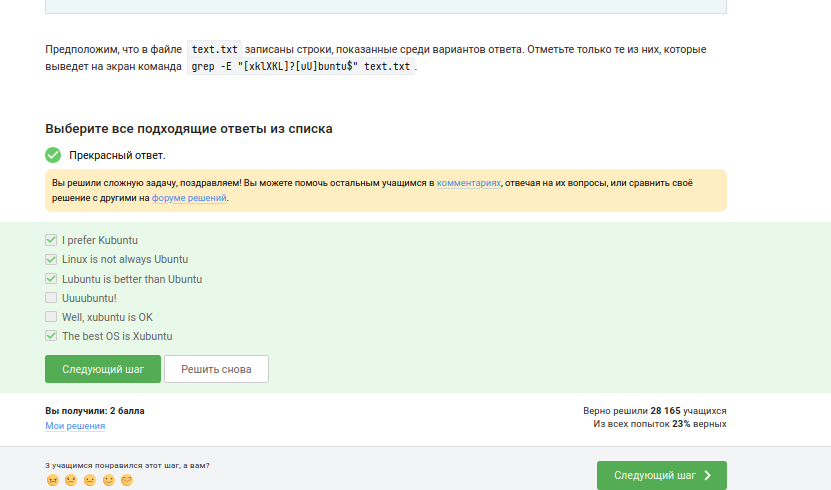
\includegraphics[width=0.7\linewidth,height=\textheight,keepaspectratio]{image3/25.png}

}

\caption{\label{fig-025}}

\end{figure}%

Без опции -n sed печатает каждую строку по умолчанию, а команда p
печатает её ещё раз. Строки, соответствующие шаблону {[}a-z{]}* (хотя бы
одна строчная буква), выводятся дважды. (рис.~\ref{fig-026}).

\begin{figure}

\centering{

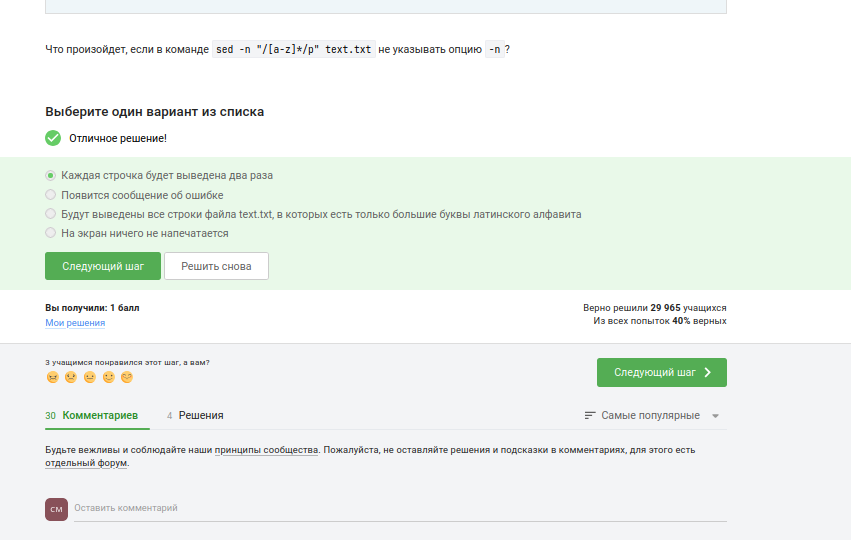
\includegraphics[width=0.7\linewidth,height=\textheight,keepaspectratio]{image3/26.png}

}

\caption{\label{fig-026}}

\end{figure}%

{[}A-Z{]}\{2,\} --- две и более заглавные буквы. g --- глобально.
Пробелы сохраняются, т.к. мы заменяем только саму аббревиатуру
(рис.~\ref{fig-027}).

\begin{figure}

\centering{

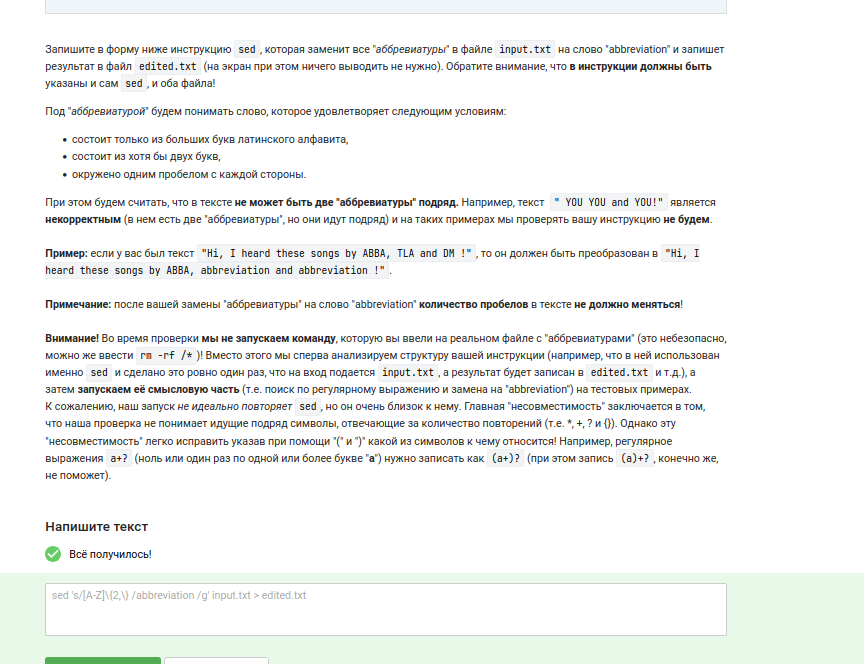
\includegraphics[width=0.7\linewidth,height=\textheight,keepaspectratio]{image3/27.png}

}

\caption{\label{fig-027}}

\end{figure}%

\section{Строим графики в
gnuplot}\label{ux441ux442ux440ux43eux438ux43c-ux433ux440ux430ux444ux438ux43aux438-ux432-gnuplot}

Опция -p (--persist) в gnuplot предотвращает закрытие окон с графиками
после завершения программы. Это удобно, когда нужно просмотреть график
после выхода из gnuplot (рис.~\ref{fig-028}).

\begin{figure}

\centering{

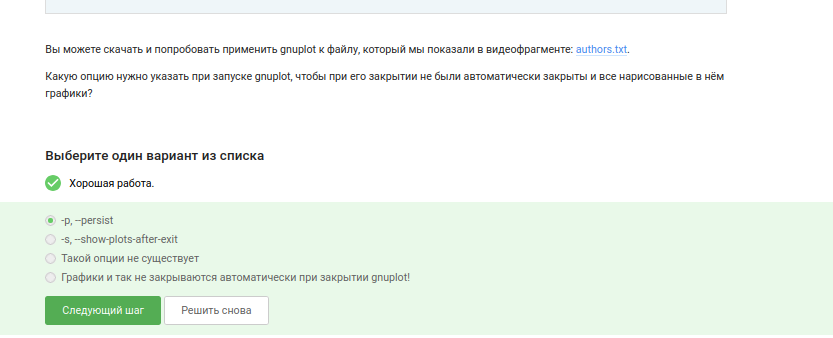
\includegraphics[width=0.7\linewidth,height=\textheight,keepaspectratio]{image3/28.png}

}

\caption{\label{fig-028}}

\end{figure}%

Правильным вариантом ответа является:

\begin{itemize}
\item
  Название -- первое значение из второго столбца, нарисовано 9 точек
  (точка из первой строки пропущена)

  \begin{enumerate}
  \def\labelenumi{\arabic{enumi}.}
  \tightlist
  \item
    Команда set key autotitle columnhead заставляет gnuplot
    принудительно интерпретировать самую первую строку файла данных как
    заголовки (названия) столбцов для легенды графика.
  \item
    По условию, в файле нет названий столбцов, там сразу идут числа (10
    строк). Из-за этой команды gnuplot всё равно заберёт первую строку
    под заголовки. Соответственно, для построения точек останется только
    9 строк.
  \item
    За отрисовку значений по вертикальной оси (оси Y) отвечает второй
    столбец (using 1:2), поэтому заголовок (имя ряда данных в легенде)
    сформируется именно из первой строки второго столбца
    (рис.~\ref{fig-029}).
  \end{enumerate}
\end{itemize}

\begin{figure}

\centering{

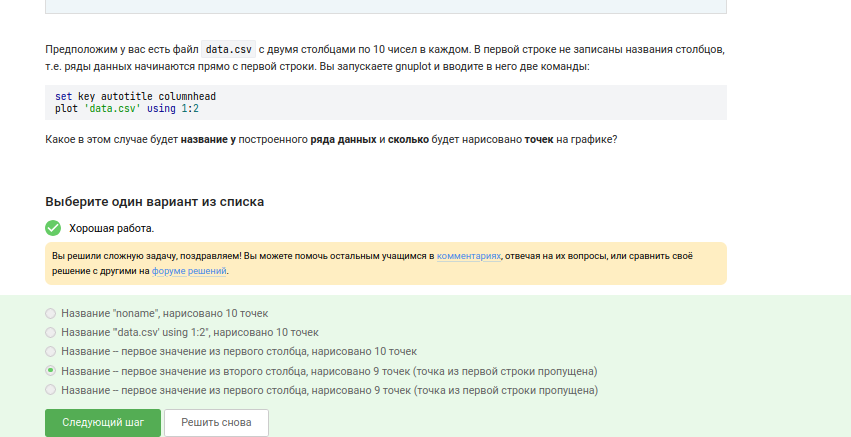
\includegraphics[width=0.7\linewidth,height=\textheight,keepaspectratio]{image3/29.png}

}

\caption{\label{fig-029}}

\end{figure}%

Команда set xtics создаёт пользовательские деления на оси X.
Конкатенация строк выполняется через точку. Например, \enquote{point 1,
value}.x1 при x1=0 даёт \enquote{point 1, value 0}, после чего
указывается координата x1.(рис.~\ref{fig-030}).

\begin{figure}

\centering{

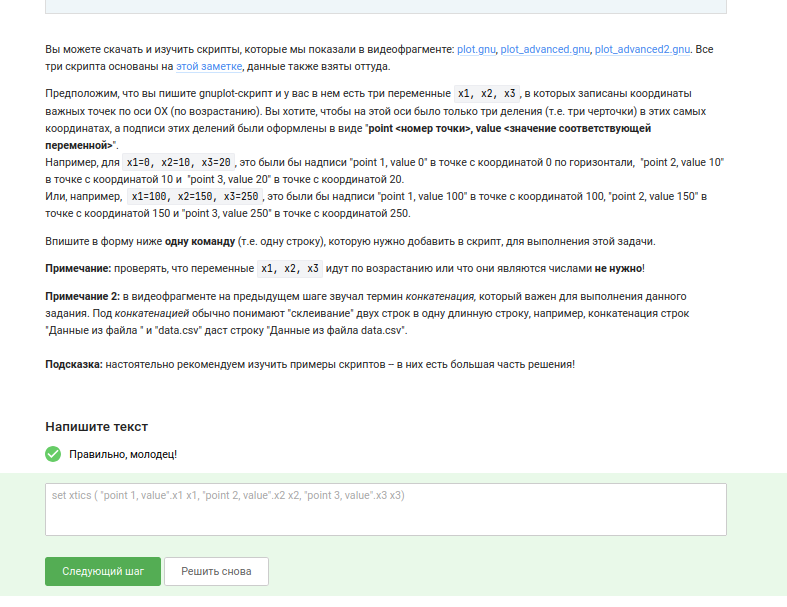
\includegraphics[width=0.7\linewidth,height=\textheight,keepaspectratio]{image3/30.png}

}

\caption{\label{fig-030}}

\end{figure}%

Для отражения графика относительно горизонтальной плоскости функция
изменена с x\^{}2+ y\^{}2 на -x\^{}2- y\^{}2. Обратное вращение
достигается изменением приращения угла: zrot = (zrot + 350) \% 360 (350
эквивалентно -10). Ускорение в два раза --- уменьшением паузы с 0.2 до
0.1 секунды (рис.~\ref{fig-031}).

\begin{figure}

\centering{

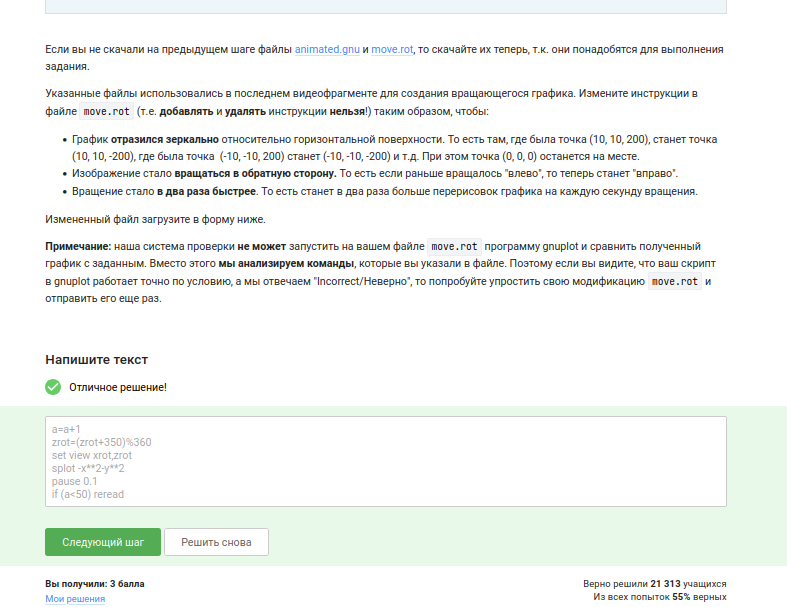
\includegraphics[width=0.7\linewidth,height=\textheight,keepaspectratio]{image3/31.png}

}

\caption{\label{fig-031}}

\end{figure}%

\section{Разное}\label{ux440ux430ux437ux43dux43eux435}

Правильными ответами для этого задания на управление правами доступа
(chmod) в Linux являются следующие варианты:

\begin{enumerate}
\def\labelenumi{\arabic{enumi}.}
\tightlist
\item
  chmod a+wx file.txt; chmod o-wx file.txt; chmod g-x file.txt
\end{enumerate}

\begin{itemize}
\tightlist
\item
  a+wx: добавляет запись и выполнение вообще всем (rwxrwxrwx).

  \begin{itemize}
  \tightlist
  \item
    o-wx: забирает их у остальных (o), возвращая к исходному r--.
  \item
    g-x: забирает выполнение у группы, оставляя ей rw-. Цель достигнута.
  \end{itemize}
\end{itemize}

\begin{enumerate}
\def\labelenumi{\arabic{enumi}.}
\setcounter{enumi}{1}
\tightlist
\item
  chmod u+wx file.txt; chmod g+w file.txt
\end{enumerate}

\begin{itemize}
\tightlist
\item
  Точечное добавление: владельцу (u) даются права на запись и запуск,
  группе (g) --- только на запись. Идеальное прямое решение.
\end{itemize}

\begin{enumerate}
\def\labelenumi{\arabic{enumi}.}
\setcounter{enumi}{2}
\tightlist
\item
  chmod ug+w file.txt; chmod u+x file.txt
\end{enumerate}

\begin{itemize}
\tightlist
\item
  ug+w: добавляет право записи (w) одновременно владельцу и группе.

  \begin{itemize}
  \tightlist
  \item
    u+x: добавляет право выполнения (x) только владельцу. В итоге
    получается нужная комбинация (рис.~\ref{fig-032}).
  \end{itemize}
\end{itemize}

\begin{figure}

\centering{

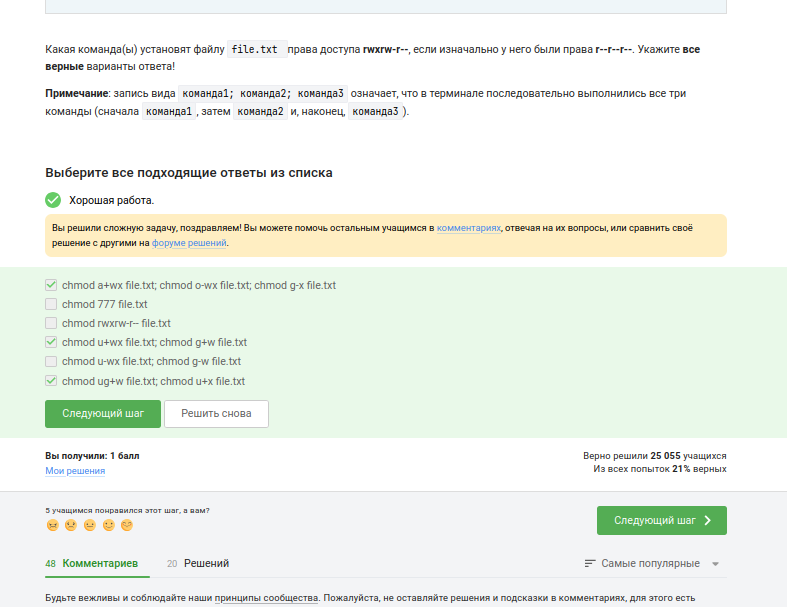
\includegraphics[width=0.7\linewidth,height=\textheight,keepaspectratio]{image3/32.png}

}

\caption{\label{fig-032}}

\end{figure}%

Изначально директория dir принадлежит пользователю root и группе root, а
её права имеют вид rwxr-xr-x (755). Наш текущий пользователь --- user,
который состоит в группе group. Чтобы user смог создавать файлы в этой
директории, ему необходимо иметь права на запись (w) в эту директорию.
Добиться этого можно несколькими путями, представленными в правильных
ответах:

\begin{enumerate}
\def\labelenumi{\arabic{enumi}.}
\tightlist
\item
  sudo chown user dir Команда меняет владельца директории на user.
  Поскольку права для владельца равны rwx (первая тройка), user
  автоматически получает полный доступ, включая возможность создавать
  файлы.
\item
  sudo chown user:group dir Аналогично предыдущему пункту, команда
  делает пользователя user владельцем (а также меняет группу на group).
  Как владелец, он получает права rwx.
\item
  sudo chmod a+w dir Эта команда добавляет право на запись (w) абсолютно
  всем пользователям (a --- all). Права директории станут rwxrwxrwx, и
  user сможет создавать в ней файлы, оставаясь в категории «остальные»
  (рис.~\ref{fig-033}).
\end{enumerate}

\begin{figure}

\centering{

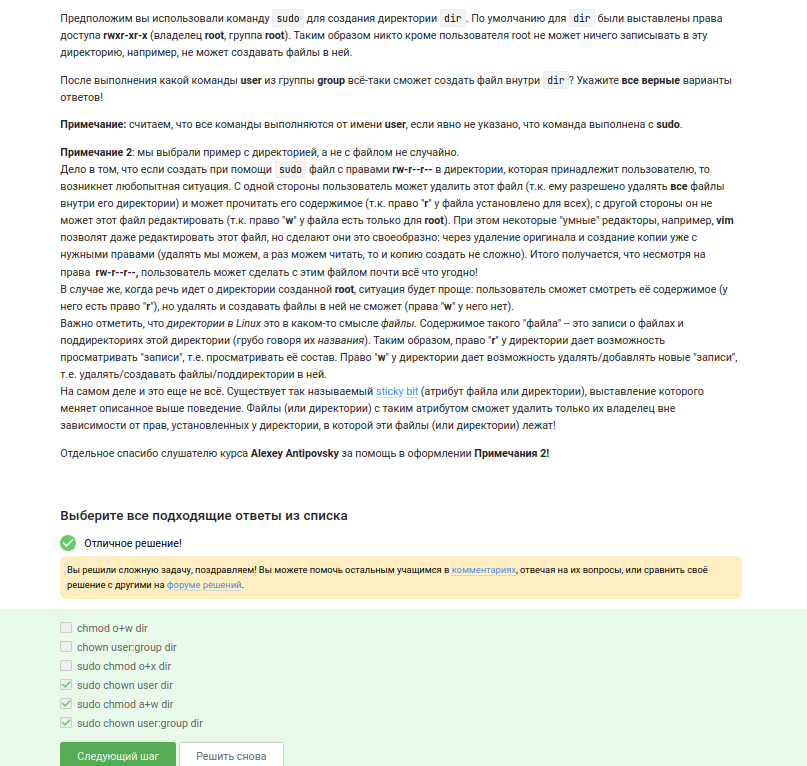
\includegraphics[width=0.7\linewidth,height=\textheight,keepaspectratio]{image3/33.png}

}

\caption{\label{fig-033}}

\end{figure}%

wc считает длину самой длинной строки, количество строк и символов, но
не считает буквы и предложения (рис.~\ref{fig-034}).

\begin{figure}

\centering{

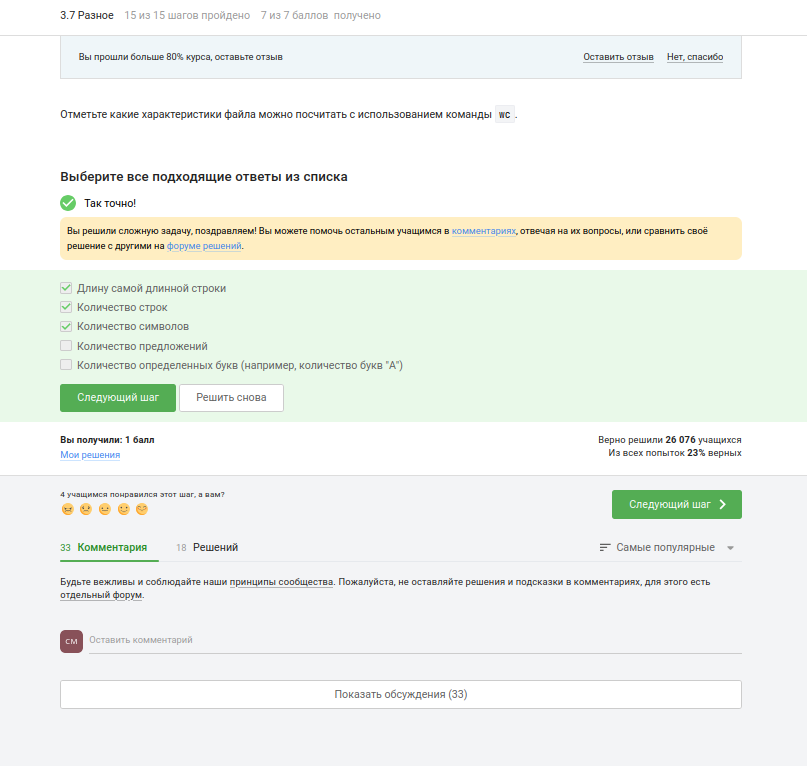
\includegraphics[width=0.7\linewidth,height=\textheight,keepaspectratio]{image3/34.png}

}

\caption{\label{fig-034}}

\end{figure}%

Команда du -sh (или du -h -s) выводит суммарный размер текущей
директории в человеко-читаемом формате (например, 2.4M). Опция -s
(summary) показывает только общий размер, без перечисления файлов
(рис.~\ref{fig-035}).

\begin{figure}

\centering{

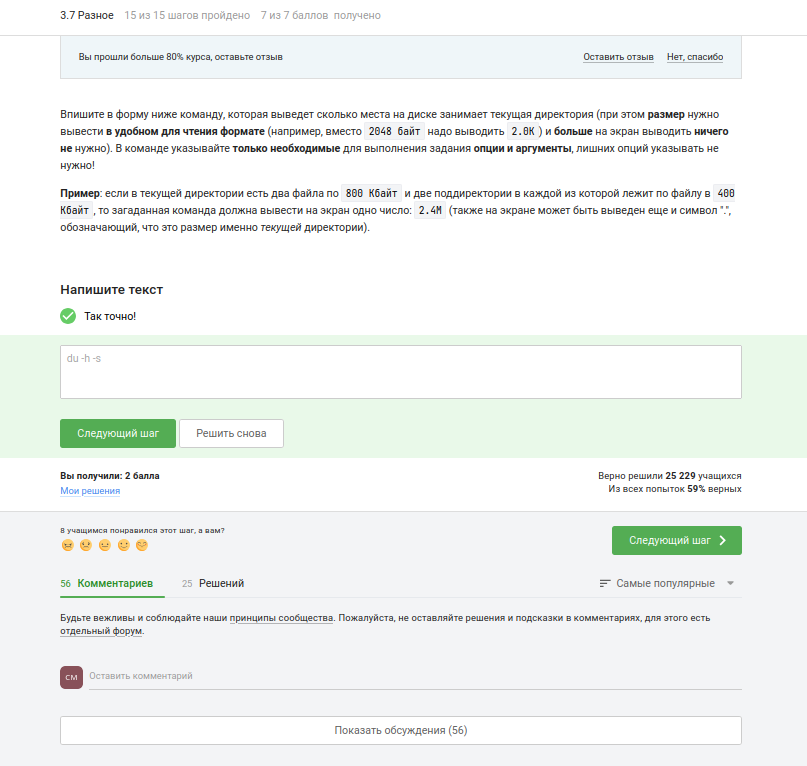
\includegraphics[width=0.7\linewidth,height=\textheight,keepaspectratio]{image3/35.png}

}

\caption{\label{fig-035}}

\end{figure}%

Самая короткая команда для создания трёх поддиректорий --- mkdir
dir\{1..3\}. Фигурные скобки в Bash генерируют последовательность: dir1,
dir2, dir3 (рис.~\ref{fig-036}).

\begin{figure}

\centering{

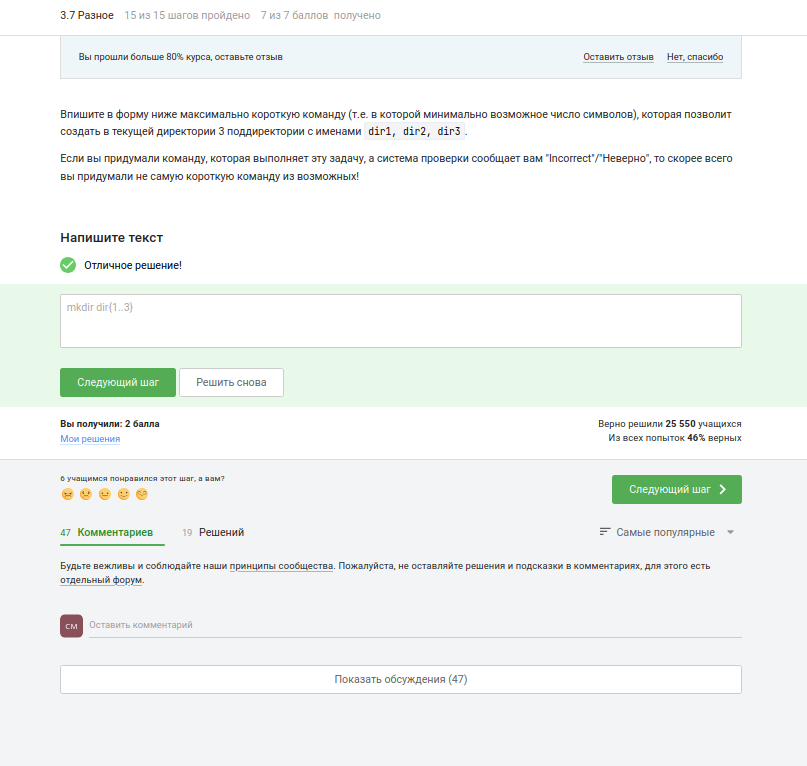
\includegraphics[width=0.7\linewidth,height=\textheight,keepaspectratio]{image3/36.png}

}

\caption{\label{fig-036}}

\end{figure}%

\chapter{Выводы}\label{ux432ux44bux432ux43eux434ux44b}

Выполнен третий этап внешнего курса на платформе Stepik.

\chapter*{Список
литературы}\label{ux441ux43fux438ux441ux43eux43a-ux43bux438ux442ux435ux440ux430ux442ux443ux440ux44b}
\addcontentsline{toc}{chapter}{Список литературы}

\printbibliography[heading=none]





\end{document}
